\documentclass[tikz,border=3pt]{standalone}
\usetikzlibrary{arrows.meta,decorations.markings}
\begin{document}
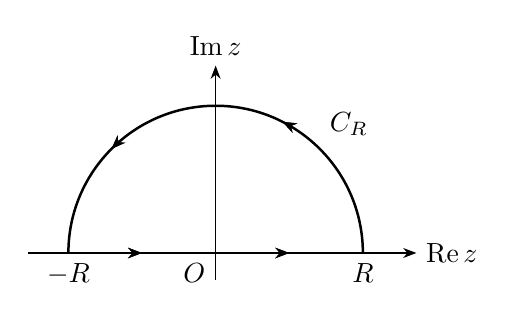
\begin{tikzpicture}[scale=0.85,>=Stealth,line width=0.9pt,
  mid/.style={postaction={decorate},decoration={markings,mark=at position #1 with {\arrow{Stealth[length=5pt]}}}}]
  % 座標軸
  \draw[line width=0.4pt,->] (-2.8,0) -- (3.0,0) node[right] {$\mathrm{Re}\,z$};
  \draw[line width=0.4pt,->] (0,-0.4) -- (0,2.8) node[above] {$\mathrm{Im}\,z$};
  \node[below left] at (0,0) {$O$};

  % 積分経路 C_R
  \draw[mid=0.25,mid=0.75] (-2.2,0) -- (2.2,0);
  \draw[mid=0.35,mid=0.75] (2.2,0) arc[start angle=0,end angle=180,radius=2.2];

  \node[below] at (-2.2,0) {$-R$};
  \node[below] at (2.2,0) {$R$};
  \node[above right] at (1.55,1.6) {$C_R$};
\end{tikzpicture}
\end{document}
